\documentclass[10pt]{article}
\usepackage{icmlko}

\icmlmeta{IP 파운데이션 월드모델}{117}{가장 큰 이득이 누수였다}{평점을 긁어 전수 검정을 돌리자 $+$0.0384 채택 4/4가 나왔는데, 그 축은 라벨을 재는 두 번째 자였다 --- 검정이 싸지면 누수도 싸게 들어온다}

\begin{document}

\twocolumn[
\icmlheader

\begin{abstract}
노트 116이 후보 스무 개를 전부 걸어 채택 0을 냈고, 스무 개의 공통점은
\textbf{전부 양(量)이거나 정적 메타}라는 것이었다. 라벨도 전부 양이다(리뷰 수 ·
서재 등록 수 · 관심 수 · 후원자 수 · 방문자 수). \textbf{평점은 다르다} ---
``본 사람들이 얼마나 좋아했나''는 ``얼마나 많이 봤나''와 다른 물리량이다.
AniList 에서 만화 1,789 · 세계애니 2,948의 평점 · 즐겨찾기 · 트렌딩을 받고,
캐시에서 모바일 · 애니 평점을 뽑아 후보 셋을 더했다(덮개율 99$\sim$100\%).
전수 검정 403초. \textbf{즐겨찾기가 $+$0.0384로 채택 4/4} --- 구간
$+$0.0352$\sim+$0.0407, 이 프로젝트 최대다. 트렌딩도 $+$0.0064 채택 4/4.
\textbf{둘 다 누수였다.} AniList \texttt{popularity} 가 만화 · 세계애니의
\textbf{라벨 그 자체}이고($\rho{=}+$1.000) 즐겨찾기가 그것과 $+$0.855로 붙는다
--- \textbf{같은 플랫폼의 같은 사용자가 매긴 두 번째 계수}였다. 트렌딩은
라벨 상관이 $+$0.505로 문턱을 빠져나가는데, 계산 자체가 그 플랫폼의 최근 목록
추가 · 투표라서 \textbf{라벨을 만든 계수기의 미분값}이다. \textbf{상관 문턱은
필요조건이지 충분조건이 아니다.} 두 겹으로 막았다 --- 라벨 상관 0.70 문턱과
\textbf{출처 차단}(라벨을 만든 계수기에서 나온 축은 상관이 낮아도 안 쓴다).
\texttt{state/sweep.py} 에 넣었다. 막고 다시 돌리니 후보 21개, \textbf{채택
0}이다. 깨끗한 것은 평점 하나뿐이고($-$0.033$\sim+$0.386, 물리량이 다르다)
$\Delta$가 $-$0.0061로 보류다. \textbf{노트 116이 ``재지 말고 걸어 봐라''로
지침을 뒤집었는데, 그 지침의 필수 짝이 이 검사다.}
\end{abstract}
]

\begin{figure*}[t]
\centering
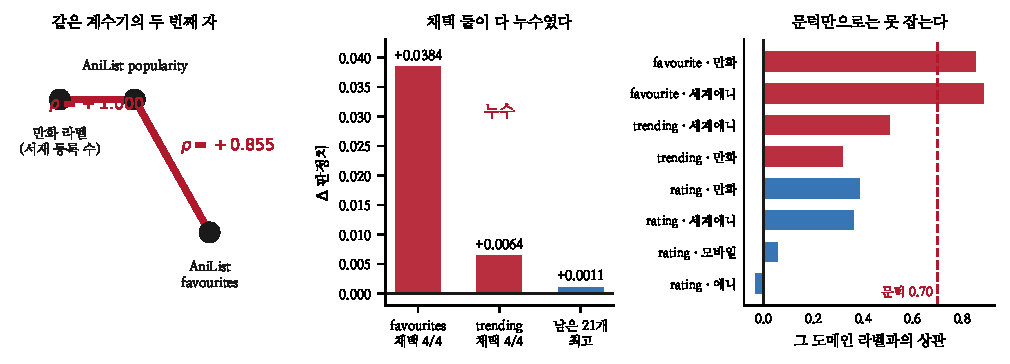
\includegraphics[width=\textwidth]{figs/lk.pdf}
\caption{왼쪽 --- 같은 계수기의 두 번째 자. 가운데 --- 채택 둘이 다 누수였다.
오른쪽 --- 문턱만으로는 못 잡는다.}
\end{figure*}

\section{다른 물리량을 긁었다}

노트 116의 후보 스무 개는 전부 \emph{양}이거나 \emph{정적 메타}였다 ---
글자 수 · 문장 수 · 밝기 · 채도 · 임베딩 성분. 라벨도 전부 양이다.
\textbf{평점은 다른 물리량이다.}

\begin{table}[t]
\centering\tsize
\caption{긁은 것. 실패 0건.}
\begin{tabular}{lrl}
\toprule
& 건수 & 출처 \\
\midrule
만화 & 1,789 & AniList meanScore · favourites · trending \\
세계애니 & 2,948 & 〃 \\
모바일 & 2,000 & 앱스토어 averageUserRating(캐시) \\
애니 & 2,073 & 라프텔 avg\_rating(캐시) \\
\bottomrule
\end{tabular}
\end{table}

\section{프로젝트 최대 이득이 나왔다}

\begin{table}[t]
\centering\tsize
\caption{전수 검정 23개 · 403초.}
\begin{tabular}{lrrl}
\toprule
& $\Delta$ & 채택 & 구간(첫 씨앗) \\
\midrule
\textbf{즐겨찾기} & \textbf{$+$0.0384} & \textbf{4/4} &
$+$0.0352 $\sim$ $+$0.0407 \\
\textbf{트렌딩} & \textbf{$+$0.0064} & \textbf{4/4} &
$+$0.0024 $\sim$ $+$0.0134 \\
\midrule
평점 & $-$0.0061 & 0/4 & $-$0.0189 $\sim$ $+$0.0030 \\
나머지 스무 개 & \multicolumn{3}{l}{노트 116과 같음(채택 0)} \\
\bottomrule
\end{tabular}
\end{table}

$+$0.0384는 노트 108의 채택($+$0.0232)보다 크고 구간이 좁다. \textbf{발표할
뻔했다.}

\section{둘 다 누수였다}

\begin{table}[t]
\centering\tsize
\caption{누수 사슬.}
\begin{tabular}{lr}
\toprule
AniList \texttt{popularity} vs 만화 라벨 & \textbf{$+$1.000} \\
즐겨찾기 vs \texttt{popularity} & $+$0.855 \\
\midrule
즐겨찾기 vs 만화 라벨 & $+$0.855 \\
즐겨찾기 vs 세계애니 라벨 & $+$0.887 \\
\bottomrule
\end{tabular}
\end{table}

\claimx{만화 · 세계애니의 라벨은 \textbf{AniList popularity 그 자체}다
($\rho{=}+$1.000). 즐겨찾기는 \textbf{같은 플랫폼의 같은 사용자가 매긴 두 번째
계수}이고 라벨과 $+$0.855$\sim+$0.887로 붙는다. \textbf{$+$0.0384는 새 정보가
아니라 라벨을 다시 읽은 것}이다.}{라벨이 popularity 라는 것은 처음부터 알던
사실이다(노트 78 · 81). \textbf{놓친 것은 같은 API 의 다른 필드가 그것의
사촌이라는 점}이었다.}

\begin{table}[t]
\centering\tsize
\caption{후보와 그 도메인 라벨의 상관.}
\begin{tabular}{lrr}
\toprule
& 상관 & 덮개율 \\
\midrule
\textbf{즐겨찾기 · 세계애니} & \textbf{$+$0.887} & 100\% \\
\textbf{즐겨찾기 · 만화} & \textbf{$+$0.855} & 100\% \\
\midrule
트렌딩 · 세계애니 & $+$0.505 & 61\% \\
트렌딩 · 만화 & $+$0.320 & 30\% \\
\midrule
평점 · 만화 & $+$0.386 & 100\% \\
평점 · 세계애니 & $+$0.363 & 99\% \\
평점 · 모바일 & $+$0.057 & 100\% \\
평점 · 애니 & $-$0.033 & 100\% \\
\bottomrule
\end{tabular}
\end{table}

\claimx{\textbf{상관 문턱은 필요조건이지 충분조건이 아니다.} 즐겨찾기는 0.70
문턱에 걸리지만 \textbf{트렌딩은 $+$0.505로 빠져나가면서 씨앗 넷을 통과한다}.
트렌딩은 그 플랫폼의 최근 목록 추가 · 투표로 계산되는 순위이므로 \textbf{라벨을
만든 계수기의 미분값}이다.}{평점도 만화 · 세계애니에서 $+$0.36$\sim+$0.39로
꽤 붙는다. 문턱을 0.35로 낮추면 평점도 걸린다 --- \textbf{문턱값 자체가
자의적}이다. 그래서 출처 차단을 함께 쓴다.}

\section{두 겹으로 막았다}

\begin{quote}\fontsize{9.0}{11}\selectfont\ttfamily
state/sweep.py \quad leak\_check()\\[.3em]
\rm ① 라벨 상관 $\ge$ 0.70 이면 뺀다\\
\rm ② \textbf{라벨을 만든 계수기에서 나온 축은 상관과 무관하게 뺀다}\\
\rm\hphantom{② }(favourites · trending · popularity)
\end{quote}

\begin{table}[t]
\centering\tsize
\caption{막고 다시 돌린 결과.}
\begin{tabular}{lr}
\toprule
후보 & 21개(누수 둘 제외) \\
시간 & 389초 \\
\textbf{채택} & \textbf{0} \\
가장 나은 것 & emb3 $+$0.0011 \\
\bottomrule
\end{tabular}
\end{table}

\begin{quote}\fontsize{9.5}{11.5}\selectfont
\textbf{노트 116이 지침을 뒤집었다} --- ``재지 말고 긁어서 걸어 봐라.''
판정이 육 분이면 그것이 옳다. \textbf{그런데 검정이 싸지면 누수도 싸게
들어온다.} 후보를 손으로 하나씩 만들 때는 그 축이 무엇인지 알고 있었는데,
API 필드를 통째로 긁어 다 걸면 모른 채로 들어온다. \textbf{빠른 검정의
필수 짝은 빠른 누수 검사다.}
\end{quote}

\section{한계}

\begin{itemize}[leftmargin=1.1em,itemsep=0.15em]
\item \textbf{채택할 것이 없다.} 누수 둘을 빼면 채택 0이다.
\item 문턱 0.70이 자의적이다. 0.35로 낮추면 평점도 걸린다.
\item 출처 차단이 이름 목록이다. 새 API 필드를 긁을 때마다 사람이 판단해
      넣어야 한다 --- 자동이 아니다.
\item 평점의 덮개율이 네 도메인뿐이다. 웹툰 · 도서 · 펀딩 · 게임 · 팝업에는
      없다.
\item ``평점은 다른 물리량''이라는 전제 자체가 만화 · 세계애니에서는 약하다
      (라벨 상관 $+$0.36$\sim+$0.39).
\end{itemize}

\section{다음}

\begin{enumerate}[leftmargin=1.3em,itemsep=0.15em]
\item \textbf{출처 차단을 자동화한다} --- 지금은 이름 목록이다. 후보를 만들
      때 ``이 필드는 어느 계수기에서 나왔나''를 함께 적게 하고, 라벨의
      계수기와 같으면 자동으로 뺀다.
\item \textbf{라벨과 다른 계수기를 찾는다} --- 이번 시도의 취지는 옳았다.
      평점은 물리량이 다르지만 \emph{같은 플랫폼}이라 절반만 다르다.
      \textbf{다른 플랫폼의 다른 계수기}가 필요하다(예: 만화의 판매 순위,
      애니의 방영 시청률).
\item \textbf{팝업 레코드} --- 열한 노트가 같은 곳을 가리킨다.
\item 텀블벅 API --- 펀딩만 미디어 홍보 0\%다.
\end{enumerate}

\vspace{0.6em}
\hrule height 0.3pt
\vspace{0.5em}
{\footnotesize
\textbf{참고문헌}\\[0.3em]
Kaufman, S. et al. (2012). Leakage in data mining: formulation, detection, and
avoidance. \emph{ACM TKDD}, 6(4), 1--21.\\[0.15em]
Cawley, G. C., Talbot, N. L. C. (2010). On over-fitting in model selection and
subsequent selection bias in performance evaluation. \emph{JMLR}, 11, 2079--2107.\\[0.15em]
Efron, B., Tibshirani, R. J. (1993). \emph{An Introduction to the Bootstrap}.
Chapman \& Hall.\\[0.15em]
Lord, F. M., Novick, M. R. (1968). \emph{Statistical Theories of Mental Test
Scores}. Addison-Wesley.\\[0.15em]
Ben-David, S. et al. (2010). A theory of learning from different domains.
\emph{Machine Learning}, 79(1--2), 151--175.
}

\end{document}
